\chapter*{PHỤ LỤC}
\addcontentsline{toc}{chapter}{PHỤ LỤC}
\setcounter{figure}{0}
\setcounter{table}{0}
\renewcommand{\thefigure}{A.\arabic{figure}}
\renewcommand{\thetable}{A.\arabic{table}}
    \section{Các linh kiện điện}
        \subsection[Cảm biến hồng ngoại TCRT5000]{Cảm biến hồng ngoại TCRT5000\footnote{Tài liệu tham khảo: \cite{vishay_tcrt5000_1}, trang 4}}
            \begin{figure}[H]
                \centering
                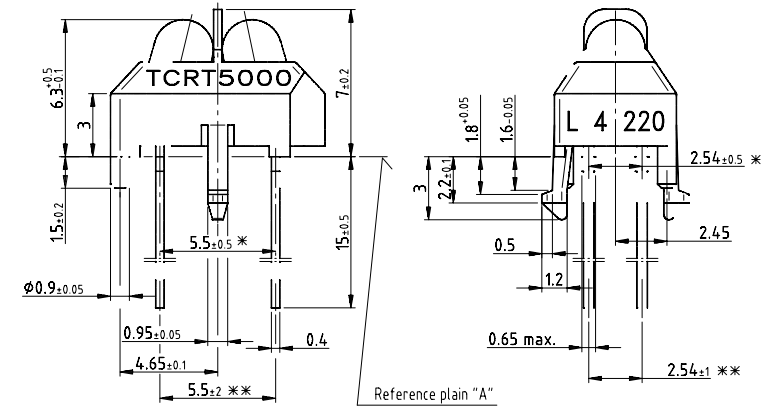
\includegraphics[width=0.88\textwidth]{pictures/appendix/app_p1_TCRT5000Dimensions1.png}
                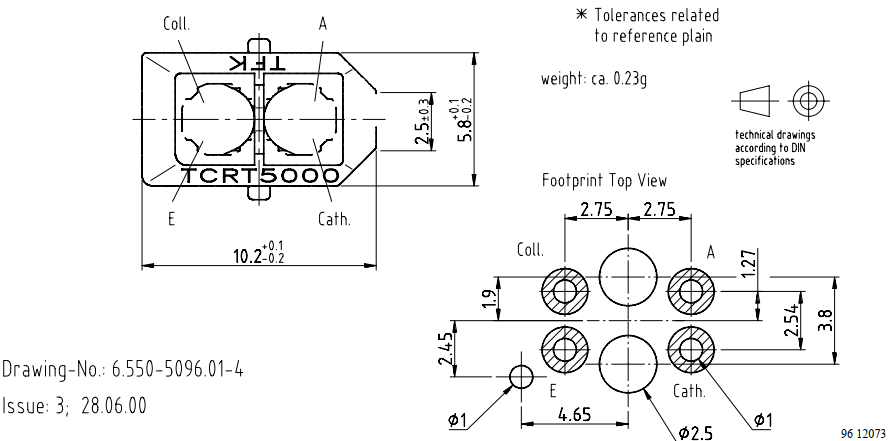
\includegraphics[width=0.88\textwidth]{pictures/appendix/app_p2_TCRT5000Dimensions2.png}
                \caption{Cảm kích thước của cảm biến hồng ngoại TCRT5000}
                \label{fig:TCRT5000}
            \end{figure}
        \subsection[Tụ điện và cuộn cảm cho mạch hạ áp]{Tụ điện và cuộn cảm cho mạch hạ áp\footnote{Tài liệu tham khảo: \cite{lm2596}, trang 25}}
            \begin{figure}[H]
                \centering
                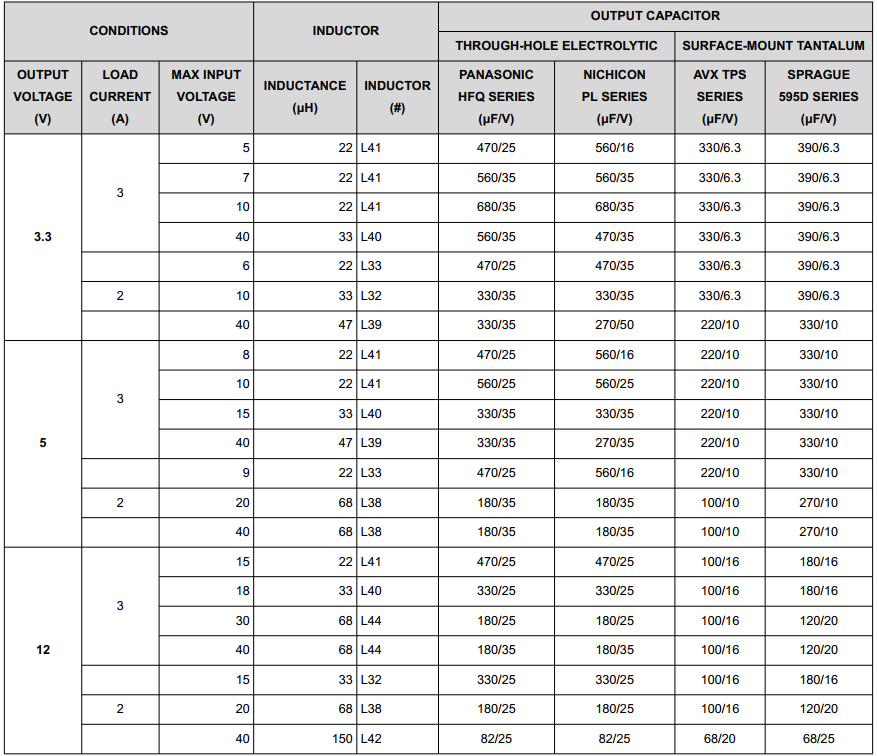
\includegraphics[width=1\textwidth]{pictures/appendix/app_p3_ChooseComponent.png}
                \caption{Cuộn cảm và tụ điện}
                \label{fig:InductorAndCapacitor}
            \end{figure}
        \subsection[Diode cho mạch hạ áp]{Diode cho mạch hạ áp\footnote{Tài liệu tham khảo: \cite{lm2596}, trang 26}}
            \begin{figure}[H]
                \centering
                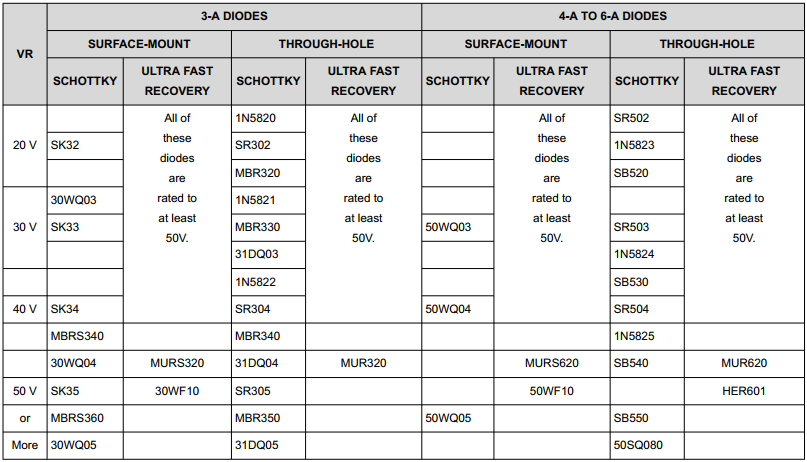
\includegraphics[width=1\textwidth]{pictures/appendix/app_p4_DiodeChoose.png}
                \caption{Diode Schottky 1N5822}
                \label{fig:Diode}
            \end{figure}

    \section{Code}
    \begin{lstlisting}[caption={Đọc file nhị phân và plot sai số e2}, label={lst:e2_plot}]
    import numpy as np
    import matplotlib.pyplot as plt

    # Config
    file_path = "data_e2_blue_16_bits.bin" 
    dt = 0.05                     # Sample time
    data_type = np.float32        # data type in buffer

    # Read file data .bin
    with open(file_path, "rb") as f:
        raw = f.read()

    # Transform to numpy array
    values = np.frombuffer(raw, dtype=data_type)

    # Create time axis
    n = len(values)
    time = np.arange(0, n*dt, dt)

    # Total time
    t_max = 20
    max_samples = int(t_max / dt)  # Number of sample

    # Plot values
    values_plot = values[:max_samples]
    time_plot   = time[:max_samples]

    plt.figure(figsize=(10,5))
    plt.plot(time_plot, values_plot, marker='o', markersize=2, linestyle='-')
    plt.title("Line tracking error e2 measured over time")
    plt.xlabel("Time (s)")
    plt.ylabel("Error e2 (mm)")
    plt.grid(True)
    plt.tight_layout()
    plt.show()
    \end{lstlisting}

        
